%%%%%%%%%%%%%%%%%%%%%%%%%%%%%%%%%%%%%%%%%%%%%%%%%%%
%
%  New template code for TAMU Theses and Dissertations starting Fall 2012.  
%  For more info about this template or the 
%  TAMU LaTeX User's Group, see http://www.howdy.me/.
%
%  Author: Wendy Lynn Turner 
%	 Version 1.0 
%  Last updated 8/5/2012
%
%%%%%%%%%%%%%%%%%%%%%%%%%%%%%%%%%%%%%%%%%%%%%%%%%%%

\documentclass[colorlinks=false,12pt]{report}
\renewcommand{\familydefault}{\rmdefault}
\usepackage[latin9]{inputenc}
\usepackage[letterpaper]{geometry}
\geometry{verbose,tmargin=1.25in,bmargin=1.25in,lmargin=1.4in,rmargin=1.15in}
\pagestyle{plain}
\usepackage[doublespacing]{setspace}
\usepackage{tocloft}
\usepackage[rm, tiny,center, compact]{titlesec}
\usepackage{indentfirst}
\usepackage{epstopdf}
\usepackage{graphicx,float,wrapfig}
\usepackage{etoolbox}
\usepackage{tocvsec2}
\usepackage[titletoc]{appendix}
\usepackage{appendix}
\usepackage{tamuconfig}
\usepackage[font=singlespacing]{caption}

% Hyperref setup below.  You should be able to get away with using uncommenting just the first line.
% \usepackage[hidelinks]{hyperref}

% if \usepackage[hidelinks]{hyperref} doesn't work try this.
% \usepackage{hyperref}  % Hidelinks is an option that removes link visiability.  TAMU Thesis Offices prefers to not see the links. But often doesn't work.  
% 
% \hypersetup{
%     colorlinks=true,
%     linkcolor=black,
%     citecolor=black,
%     filecolor=black,
%     urlcolor=black,
% }
%%%%%%%%  End of hyperref setup.  One of these two options should work, but my motto with hyperref is when in doubt, comment it out!

\begin{document}
\renewcommand{\tamumanuscripttitle}{FIXME Location Prediction Based on Tie Strength}
\renewcommand{\tamupapertype}{Dissertation}
\renewcommand{\tamufullname}{Jeffrey Allen McGee}
\renewcommand{\tamudegree}{Masters of Science}
\renewcommand{\tamuchairone}{James Caverlee}
% Uncomment out the next line if you have co-chairs.  You will also need to edit the titlepage.tex file.
%\newcommand{\tamuchairtwo}{Additional Chair Name}
\renewcommand{\tamumemberone}{Frank Shipman}
\newcommand{\tamumembertwo}{Daniel Sui}
\renewcommand{\tamudepthead}{Hank Walker}
\renewcommand{\tamugradmonth}{December}
\renewcommand{\tamugradyear}{2012}
\renewcommand{\tamudepartment}{Computer Science}


\include{titlepage} % This is simply a file that formats and adds your titlepage, please do not edit this unless you have a specific need. .
%%%%%%%%%%%%%%%%%%%%%%%%%%%%%%%%%%%%%%%%%%%%%%%%%%%
%
%  New template code for TAMU Theses and Dissertations starting Fall 2012.
%  For more info about this template or the
%  TAMU LaTeX User's Group, see http://www.howdy.me/.
%
%  Author: Wendy Lynn Turner
%	 Version 1.0
%  Last updated 8/5/2012
%
%%%%%%%%%%%%%%%%%%%%%%%%%%%%%%%%%%%%%%%%%%%%%%%%%%%
%%%%%%%%%%%%%%%%%%%%%%%%%%%%%%%%%%%%%%%%%%%%%%%%%%%%%%%%%%%%%%%%%%%%%
%%                           ABSTRACT
%%%%%%%%%%%%%%%%%%%%%%%%%%%%%%%%%%%%%%%%%%%%%%%%%%%%%%%%%%%%%%%%%%%%%

\chapter*{ABSTRACT}
\addcontentsline{toc}{chapter}{ABSTRACT} % Needs to be set to part, so the TOC doesnt add 'CHAPTER ' prefix in the TOC.

\pagestyle{plain} % No headers, just page numbers
\pagenumbering{roman} % Roman numerals
\setcounter{page}{2}

\jam{limit of 350 words}

\indent With the rise of volunteered user location information through services
like Foursquare, Google Latitude, and Facebook Places, we face unprecedented
access to the real-world connections among millions of social media users.
%
This location information is increasingly incorporated into social media for
providing localized content, location-aware recommendations, and other
geo-spatial enabled services.
%
In this paper, we investigate the relationship between the strength of the tie
between a pair of users, and the distance between the pair through an
examination of over 100 million geo-encoded tweets and
over 73 million user profiles collected from \temp{information publicly
posted to} Twitter.
%
Based on this investigation, we identify several factors such as number of
followers and how the users interact that can strongly reveal the distance
between a pair of users, and use these factors to train a decision tree to
distinguish between users who are likely to live nearby and pairs of users who
are likely to live in different areas.
%
We use the results of this decision tree as the input to a maximum likelihood
estimator to predict a user's location.
%
We find that this proposed method significantly improves the results of
location estimation relative to a state-of-the-art technique.
%
Our system reduces the average error distance for 80\% of Twitter users from 40
miles to 21 miles using only information from the user's friends and
friends-of-friends.

\pagebreak{}

%\include{dedication}
%%%%%%%%%%%%%%%%%%%%%%%%%%%%%%%%%%%%%%%%%%%%%%%%%%%%
%
%  New template code for TAMU Theses and Dissertations starting Fall 2012.  
%  For more info about this template or the 
%  TAMU LaTeX User's Group, see http://www.howdy.me/.
%
%  Author: Wendy Lynn Turner 
%	 Version 1.0 
%  Last updated 8/5/2012
%
%%%%%%%%%%%%%%%%%%%%%%%%%%%%%%%%%%%%%%%%%%%%%%%%%%%


%%%%%%%%%%%%%%%%%%%%%%%%%%%%%%%%%%%%%%%%%%%%%%%%%%%%%%%%%%%%%%%%%%%%%%
%%                           ACKNOWLEDGEMENTS
%%%%%%%%%%%%%%%%%%%%%%%%%%%%%%%%%%%%%%%%%%%%%%%%%%%%%%%%%%%%%%%%%%%%%
\chapter*{ACKNOWLEDGEMENTS}
\addcontentsline{toc}{chapter}{ACKNOWLEDGEMENTS}  % Needs to be set to part, so the TOC doesnt add 'CHAPTER ' prefix in the TOC.

I want to start by thanking my parents, Gary and Susan McGee, for their
support and encouragemet over the years.
%
They laid the foundation of my education.
%
I am grateful to my advisor, Dr. Caverlee, for everything he did to support my
research.
%
He taught me to research, to analyze data, and how to really read a reasearch
paper.
%
Jeremy Kelly introduced me to Infolab, and founded a handful of companies
that employed me on and off during my years of graduate school.
%
His mentorship made me a better software developer.
%
I'd like to thank Brian Eoff for building the Twitter Streaming API client that
downloaded the initial set of geo-located Tweets.
%
Zhiyaun Cheng deserves credit for his work on the problem of location detection
and for reccomending quite a few papers to me.
%
Many thanks to Krishna Kamath, Elham Khabiri, Kyumin Lee, Yuan Liang, and the
rest of Infolab.
%
And finally, my thanks are due to my awesome wife Keri Bean.
%
Her love and encouragement helped me to finish this journey.
\pagebreak{}

%\include{nomenclature}
%\include{lists}  % This is simply a file that formats and adds your toc, lof, and lot, please do not edit this unless you have a specific need. .

\ifdefined\THESIS
    \pagestyle{plain} % No headers, just page numbers
    \pagenumbering{arabic} % Arabic numerals
    \setcounter{page}{1}
    \chapter{\uppercase {Introduction and Related Work}}
\else
\fi

\section{Introduction}

Online social networks are increasingly getting ``geographical.'' Millions of online
social network users are voluntarily sharing their location through location sharing
services like Foursquare, short text status updates
through real-time microblogs, and photos in online image hosts. This location
information is increasingly being
incorporated in social media for providing localized content, location-aware
recommendations, and other geo-spatial enabled services. The access to the
trails and connections among millions of social media users provides an
unprecedented opportunity to study the relationship between the geographical
properties of social media users and the social relations connecting them.

With high-quality geographic information, online services become more useful to
the local community.  Online services can bring to light discussions about what
the city council voted on last night.  Online services can identify, and react
to, the crowd of people gathering for the big football game.  Online services
can do a better job suggesting friends.  Online services can reconnect users
with the community that the users neglected when they started spending their
time online.

Geographic information is also useful for researchers.  In the past few years,
there has been growth in research into topics such as geographical user
clustering and location-based social networks.  As the accuracy of geographic
information improves, it will open up new research opportunities.

In this paper, we investigate the interplay of distance and tie strength
through an examination of FIXME million geo-encoded tweets and FIXME million user
profiles collected from Twitter. Concretely, we investigate the relationship
between the strength of the tie between a pair of users and the distance
between the pair.  We identify several factors -- including following,
mentioning, and actively engaging in conversations with another user -- that
can strongly reveal the distance between a pair of users.

FIXME: bimodal?

We find a bimodal distribution in the distance between Twitter users, with one
peak around 10 miles from people who live nearby, and another peak around 2500
miles, further validating Twitter's use as both a social network (with
geographically nearby friends) and as a news distribution network (with very
distant relationships).  Figure~\ref{fig:EdgeTypes} gives a preview of this
bimodal distribution for four basic types of relationships.  The red curve
represents a strong, reciprocal friendship whereas the cyan line represents a
relatively weak relationship. The red curve has more users at a distance of ten
miles than the cyan line, indicating that reciprocal friendships are more
likely to be local.

Based on these findings, we propose and evaluate a framework for predicting
location for users based on an analysis of the user's social network,
which has great significance for augmenting traditional social media and
enriching location-based services with more refined and accurate location
estimates.  FriendlyLocation correctly locates FIXME\% of users within 25 miles.

\section{Related Work}

%FIXME: Mr. Cheng wrote some of this.

The study of geographical properties of online social media users has drawn
intensive attention in recent years.  Characterizing network properties in
relation to local geography has been studied in \cite{yardi2010tweeting}.
Lindqvist \cite{lindqvist2011m} analyzed how and why people use location
sharing services, and discussed the privacy issues related to location sharing
services.

Scellato et al. \cite{scellato2011socio} used data from three location based
social networks to investigate the relationship between distance and location,
and they show that connections are not purely caused by geographical or social
factors.  They investigated two random models where they shuffle the user
locations and another where they shuffle the social connections and investigate
what happens to the user location.  They show that if a user has more
connections, then their friends tend to be further away.  They also found that
longer connections are equally likely to be part of a social triangle as
shorter connections.

We know of two previous systems that attempted to estimate the location of
users on social networking sites.  In the first, Facebook researchers analyzed
the physical distance between Facebook users' social relations and utilized the
locations of a user's friends' to predict the user's geographical location
\cite{backstrom2010find}.  They picked users who entered their street address
in the location field of their profile and used this to predict the location of
their friends using maximum likelihood estimation.  However, the information
they used is generally not available outside of Facebook, since people rarely
make their street address public.  Cheng et al. \cite{cheng2010you} propose a
content-based system for locating users on Twitter. They find words that are
highly concentrated in specific regions and build a model to calculate the
probability that a user lives at a location.

FIXME: add new papers here - especially the twitter ones

Gilbert \cite{gilbert2009predicting} shows how the strength of a tie can be
predicted by interaction patterns.  They had volunteers rate the strength of
several friendships and then analyzed the activity between the users can
predict the strength of the friendship.  We argue that tie strength is also
correlated with physical proximity.

There has also been some research into specific aspects of Twitter that is
relevant to our work.  User behavior with regard to the location field in
Twitter user profiles has been studied in \cite{hecht2011tweets}.  One of the
early investigations into Twitter usage by Java \cite{java2007we} showed that
people use twitter for chatter, conversations, sharing information, and
reporting news.  This mixture of uses fits well with the bimodal distribution
of friends and followers that we propose.

Finally, Cranshaw et al. \cite{cranshaw2010bridging} solved the inverse of the
problem we are investigating: they predicted the existence of a social network
tie given precise location information from laptops and cell phones. They used
a collection of features of when users are co-located.  Together, these efforts
have begun to lay a foundation for the study \textit{geo-social media}.


\chapter{\uppercase {Data Collection}}

Text goes here.

\section{Crawling}
To investigate how social relation and geographical distance between the
relations correlate, we sample a dataset from Twitter.
Before going into the details of the data collection, we first define a few
terms to simplify the process of explaining how the data was collected.
\textbf{Contacts} are defined to be the set of a user's friends, followers, and
people who a user mentioned in her tweets (i.e., people the user speaks to). 
Twitter does not provide a mechanism to determine who mentioned a given user.
Thus, only one-directional conversation is considered.
In some blogging platforms, such as Tumblr, it is relatively easy to find the
communication edges that point back toward a user.
In those platforms, it would be fairly straightforward to use that information in location prediction.

Any given contact can be categorized into precisely one of these four disjoint sets:
\begin{description}
\item[reciprocal friend] The geo-located user follows this user and is followed back.
\item[just friend] The geo-located user follows this user and is not followed back.
\item[just follower] The geo-located user is followed by this user, but does not follow them.
\item[just mentioned] The users do not follow each other, but the geo-located user mentioned the name of the other user in a tweet.
\end{description}

We built a crawler to find these contacts for users who used Twitter's Location
Feature to disclose their location.
The crawler sampled 19,877,804 geo-coded tweets by monitoring Twitter's public
Streaming API between April 7 until April 16, 2011.
In the dataset, users are filtered who have strict privacy settings, have
neither friends nor followers, or posted fewer than two tweets in the sampled
dataset.
For each user in the geo-coded tweets, we use the median latitude and median
longitude of locations of the user's tweets as an approximation of her home
location. 
Some Twitter accounts, such as accounts that posted jobs, would
move around faster than a human could possibly move. To account for this, the crawler
calculated the distance between each tweet and the user's home location. The crawler
ignored users if the median distance from their tweets to their home location
was greater than 50 miles.

Users are considered to be in the US based on a simple bounding box.  If their
median latitude was between 24 and 50 degrees and their median longitude was
between -126 and -66 degrees, then their home location was considered inside
the continental US.
We divided these geo-located users into groups based on the last digit of their twitter user id:
\begin{description}
\item[Training (0--6)] 104,214 users with a home location in the US bounding
box. Some of these users were also used to evaluate the quality of geocoding.
For geocoding, we chose users from around the world with a decodable location
field and split them into two groups:
\begin{description}
\item[Geocoding Training (0--3)] 131,295 users
\item[Geocoding Evaluation (4--6)] 85,664 users
\end{description}
\item[Evaluation (7--9)] 40,861 users with a home location in the US.
\end{description}

For all of the geo-located users with a home location in the US, the crawler
used Twitter's API to download the users' friends, followers, and 100 most
recent tweets.
The crawler also downloaded the profiles for up to 2000 friends, followers, and
people they mention in their tweets. If they had over 2000, it chose a random
sample of 2000 profiles that included at least 25 of each of the four
categories listed below.
From the profiles, the crawler kept the users with a decodable location field
and threw away the rest. From what was left, the crawler randomly picked one
Friend, one Follower, one Just Mentioned, and up to seven reciprocal friends.
For each of these contacts, the crawler stored their friends, followers, and 100 most recent tweets.

\section{Geocoding}
%We used Gisgraphy\footnote{\url{http://www.gisgraphy.com/}} to do geocoding.
%Gisgraphy does full-text search on the GeoNames\footnote{\url{http://www.geonames.org/}}
database using Lucene. Since
it runs locally it is not limited to a certain number of queries per day.
Gisgraphy's geocoder returns ranked results based on a full text search
over millions of geographical features such as countries, cities, and schools. 

The location field on a user's profile is just a text field that asks the user
to respond to ``Where in the world are you?''.
Responses vary from precise latitude and longitude coordinates entered
automatically by smart phone apps to jokes and nonsense.
Our system does some preprocessing before sending user-submitted locations to
the geocoder.
First, it uses a regular expression to find latitude and longitude coordinates.
These are treated as if they were a unique type of location returned by the
geocoder.
Occasionally, users would put two locations separated by a slash, dash or a
conjunction. If the geocoder did not return any results for a user, our system tried to
geocode both locations and returned the first location that the geocoder
understood.

Some locations are significantly more useful than others.
For example, even though Rhode Island and Montana are both states with around
one million people, Rhode Island is smaller, and as a result, much more useful
in estimating the location of a user.
To make the results of the geocoder more useful, we devised a method to
estimate the accuracy of a location returned by the geocoder.
Because users in the US had friends outside of the US, FriendlyLocation needs
to estimate the quality of
locations outside of the US as well.
As a result, we trained the geocoder trained on geographic data from around the world.

\begin{table}[t]
\centering
\caption{Example Median Location Errors (miles)}
\begin{tabular}{l r r} 
Location&Number of Users&Median Error\\ \hline
``Bronx''&53&4\\
``New York''&1264&174\\
``Pluto''&11&7843\\ \hline
\\
Place Type&Number of Users&Median Error\\ \hline
(latitude, longitude)&25216&3\\
A City&7128&6\\
An Airport&117&31\\
A Country&37&3935\\
\hline\end{tabular}
\label{tab:MedianLocErr}
\end{table}

For the users in the geocoding training and evaluation groups, we have both the
home location based on geo-located tweets, and the free-response location field
that the geocoder was able to decode.
We define the \textbf{location error} to be the great circle distance between a user's home
location and the location returned from the geocoder.
The location error can vary from less than a mile to over ten thousand miles.
Each user in the geocoding training group was geocoded and grouped based on the exact location returned by the geocoder.
For the 3866 locations that had at least three users, we calculated the median location error for that location.
All the users who were at locations with only one or two users were grouped
according to the type of location returned by the geocoder.
We calculated the median error for each location type.
The median is more appropriate than the average or standard deviation because
those metrics are strongly affected by large outliers.
We choose to make the cutoff three because that is the smallest value where the median is not just an average.
Table \ref{tab:MedianLocErr} shows the median location error for a few example locations and location types.

This gives us a method to estimate the quality of a coordinate returned by Gisgraphy.
We define the \textbf{predicted location error (PLE)} for a given location to be the
median location error if it is one of the 3866 locations that had three users;
otherwise, it is the median location error for the location's type.
For example one user had ``PDX,OR'' in his location field. Gisgraphy identifies
this as ``Portland International Airport''. Since it is not one of the most
common locations, its PLE is determined by its place type to be 31 miles as
seen in Table \ref{tab:MedianLocErr}.

Figure \ref{fig:DiffGnpGps} shows the result of using the PLE to ignore users
who have low quality locations such as ``Pluto''.
The solid black line represents the normal results of geocoding where the
location error is less than 1000 miles for 88\% of the users.
The cyan line shows the results of removing locations with a PLE greater than
or equal to 1000 miles.
After removing only 6\% of the users, 93\% of them are within 1000 miles.

\ifdefined\THESIS
    \chapter{\uppercase{Analysis of Distance to Contacts}}
\else
    \section{Analysis of Distance to Contacts}
\fi

% FIXME: For each subsection finding (e.g., "What is the distribution of
% contacts?") you need to add more intuition/analysis. Walk the reader through
% each figure. Highlight some actual numbers from the figures in the text. Tell
% us what those numbers mean. Tell me what I should learn. You do some of this
% already, but it really needs to be expanded. Remember, your reader is not as
% on top of this material as you are, so you need to do more handholding.


% FIXME: For all figs, I think you may need a black/white legible version. I'm
% worried about readers seeing lots of lines and not wanting to go back to the
% screen PDF to tell the difference. What did Backstrom do for their FB paper?

% FIXME: For all figs, you might want to add a takeaway sentence in the
% caption. So if a reader only looks at the fig (without following along in the
% text), they can learn something.

Every user who has multiple contacts will have some contacts who are much
closer than others. In order to estimate the locations of users, we would like
to find out which users are most likely to live nearby.  In this section, we
investigate how various types of contacts correlate with proximity.
All of the analysis in this section was done on the contacts of 249584 geo-located users.
Contacts with a predicted location error that was greater than or equal to 1000
miles were filtered out.

\subsection{What type of contact is closest?}
\label{sec:EdgeTypes}

\begin{figure}[tb]
\centering
\includegraphics[width=\linewidth]{figures/edge_types_cuml.pdf}
\caption{
CDF of distance from geo-located users to users they have some contact
with.
}
\label{fig:EdgeTypesCum}
\end{figure}

FIXME: add US-only line to one of these graphs for comparison to other papers

Figure~\ref{fig:EdgeTypesCum} shows the cumulative distribution
function(CDF) of the distance between a geo-located user and several types of
contacts.
Distance is plotted on a logarithmic scale to show both local and
global effects.

In general, reciprocal friends are the closest, followed by followers, friends,
and finally users who are just mentioned.
37\% of reciprocal friends live within 25 miles while only 18\% of users
who are just mentioned live within that radius.
While it may seem that since being followed by someone and following someone
should be identical, they are not.
Celebrity and news accounts on Twitter often have large numbers of followers,
but they normally do not follow a large number of users.
Since the geo-located user was selected randomly, they are usually an average
user and not a celebrity.
If they follow someone, it might be a celebrity; however, if someone follows
them, it is probably someone who knows them.

\subsection{What is the distribution of contacts?}

\begin{figure}[tb]
\centering
\includegraphics[width=\linewidth]{figures/edge_types_norm.pdf}
\caption{
Histogram of distance to users for different types of relationships.
The curves in this figure are the derivatives of the curves in
Figure~\ref{fig:EdgeTypesCum}.
}
\label{fig:EdgeTypes}
\end{figure}

To understand the distribution of contacts, we created a histogram of the distances between various types of contacts.
We sorted the distances to contacts into 200 logarithmically
scaled bins (40 bins for each power of 10).
Figure~\ref{fig:EdgeTypes} shows the result of plotting the histogram.
%
All four types of contacts follow roughly the same
distribution: one peak around 10 miles from people who live nearby, and several
other peeks between 100 and 10,000 miles. These peeks occur at the distances
between major population centers.

% FIXME: The comment on Twitter being a news distribution network should cite
% that WWW paper from Moon that examines exactly this question.

One reasonable explanation for this is that Twitter is not just a social
network; it is also a news distribution network.  This distribution
suggests that users have two types of contacts: people who they met in
real life, and people who they met online or know about via mainstream media.
The former group is useful for predicting location and the latter group is not.
In section~\ref{sec:model}, we use this idea that there are two types of
contacts to build a predictive location model based on social ties.


\ifdefined\THESIS
    \begin{figure*}[tb]
    \subsection{Are users closer to people they communicate with?}
    \centering
    \includegraphics[width=\linewidth]{figures/com_types.pdf}
    \caption{
    CDF of the distance between a geo-located user and various types of contacts
    piloted on a logarithmic scale.
    }
    \label{fig:ComTypes}
    \end{figure*}
\fi

\begin{table*}[tb]
\centering
\begin{tabular}{l | r r | r r | r r | r r}
    & \multicolumn{2}{c}{I Talk}
    & \multicolumn{2}{|c}{We Talk}
    & \multicolumn{2}{|c}{You Talk}
    & \multicolumn{2}{|c}{We Ignore} \\
    \cline{2-9}
    &local&count&local&count&local&count&local&count \\
    \hline
    Just Follower & 40\%&2001 & 47\%&792 & 40\%&5958 & 25\%&216834 \\
    Recip Friend & 42\%&28067 & 50\%&17903 & 45\%&21066 & 35\%&168973 \\
    Just Friend & 21\%&23314 & 40\%&910 & 42\%&1884 & 21\%&212969 \\
    Just Mentioned & 18\%&182978 & 36\%&4721 & & & & \\
\end{tabular}
\caption{
FIXME: explain this
The effect of communication on tie strength.
In these graphs, ``I'' refers to the geo-located user. ``You'' refers to their
contact.
}
\label{tab:ComTypes}
\end{table*}


Table~\ref{tab:ComTypes} shows the relationship between various types of
communication patterns between the geo-located users and their contacts.
In almost every case, increased communication increases the probability that
two users live near each other.
There is one exception: when an average user mentions someone they follow who
does not follow them back, it has no effect.
In other words, if a random user mentions a celebrity who does not bother to
reply, they probably do not live in the same area. This can be seen by the blue
and green lines that are right on top of each other in the Just Friend graph.
On the other hand, in the rare event that someone who is just a friend replies
to their follower, then the probability that they live near each other is much
higher.

The weakest type of contact is for users who were just mentioned, but never
replied to. If the person is mentioned, then 36\% of users with no
friend/follow relationship who have a conversation live within 25 miles.
This is approximately equal to the 35\% of reciprocal friends who ignore each
other and live within 25 miles.
Unsurprisingly, the strongest type of connection is reciprocal friends who
communicate.


\subsection{Are users closer to private accounts?}

\begin{table}[tbh]
\centering
\begin{tabular}{l | r r | r r}
    & \multicolumn{2}{c}{Public}
    & \multicolumn{2}{|c}{Private} \\
    \cline{2-5}
    &local&count&local&count \\
    \hline
    Just Follower & 25\%&204417 & 31\%&21168 \\
    Recip Friend & 37\%&211136 & 41\%&24873 \\
    Just Friend & 21\%&233849 & 39\%&5228 \\
    Just Mentioned & 18\%&183368 & 35\%&4331 \\
\end{tabular}
\caption{
    Private accounts tend to be closer.
}
\label{tab:EdgeTypesProt}
\end{table}

Like many social networks, Twitter allows users to mark their account as
protected. The specifics differ from network to network, but in Twitter's case
a user has to be approved to follow a protected user.
There are demographic differences between public and protected accounts.
For example, Gilbert \cite{gilbert2008network} demonstrates that rural users
are more likely to make their accounts private than public accounts.
In the case of protected accounts on Twitter, basic information
about their profile such as their location and the number of friends and
followers is public, but their friends list, followers list, and the text of
their tweets is private, and not available for analysis.

As seen in Table~\ref{tab:EdgeTypesProt}, the most dramatic difference between
private and public occurs if a user follows a protected account.
%
Since users generally only allow people they know to follow a protected
account, this brings the users almost as close together as if they were
reciprocal friends.
%
On the other hand, if a protected account follows the geo-located user, they
are only slightly more likely to be nearby.

\subsection{If two of your friends live near each other, does that increase the
chance that they live near you?}

\begin{figure}[tb]
\centering
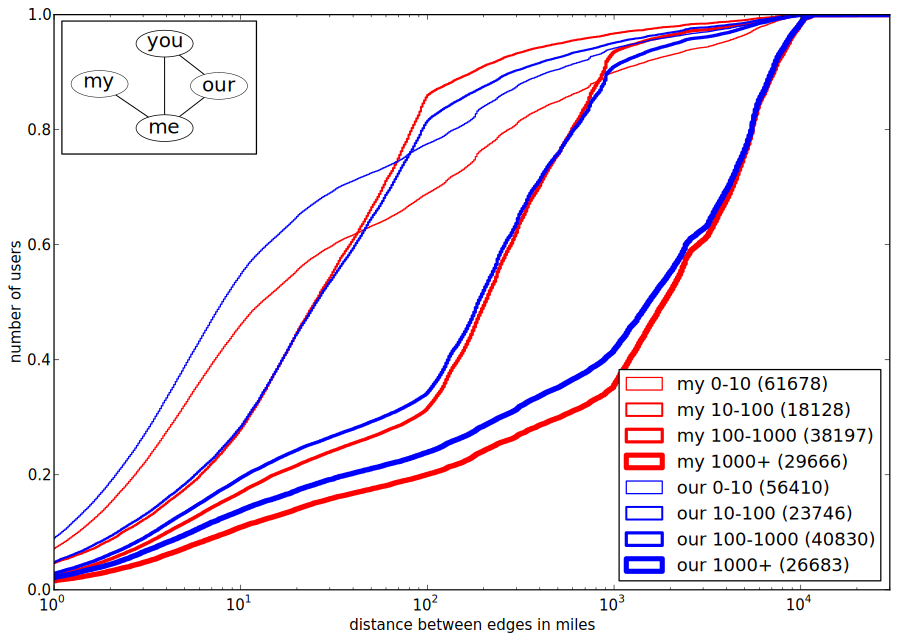
\includegraphics[width=\linewidth]{figures/near_triads.pdf}
\caption{
Comparison between distance to a mutual friend, labeled ``our'', and someone
who is not a mutual friend, labeled ``my''.
The figure in the upper-left corner shows the shape of the social graph we used
to create this graph.
}
\label{fig:NearTriads}
\end{figure}

In this section, we turn our attention to triangles of users.
Finding useful relationships between the edges of a social triangle is tricky
because the three distances depend on each other.
Unfortunately, it is fairly simple to show using the triangle inequality theorem
that if two users are 1000 miles apart, then the third member of the triangle
has to be at least 500 miles from one of the other two.
Since this isn't a useful result, we designed a more complex experiment to
analyze the relationship between the sides of the triangle.
A script searched for a specific pattern in the social network of the
reciprocal friends.  It needed four users who fit the following criteria:
\begin{itemize}
\item ``me'' is the geo-located user
\item ``you'' is reciprocal friends with ``me''
\item ``my'' has no relationship with ``you'' and is reciprocal friends with ``me''
\item ``our'' is reciprocal friends with both ``me'' and ``you''
\end{itemize}

% FIXME: when you talk about the me, you, my, our. I would put that subfigure
% from the figure in the body of the text so it is clearer. And the language
% itself is pretty tough to follow. Not sure on how to improve it, but it is
% confusing.

We found this pattern for 147669 of the geo-located users.
If a user had multiple instances of this pattern, it picked one of them
randomly so that particular users would not bias the results.
Since our crawler only retrieved friend and follower information for at most
seven reciprocal friends per user, it is reasonable to assume that this pattern
is much more common, but the sample is more than enough data to draw some
conclusions.

Figure~\ref{fig:NearTriads} shows a comparison between the ``my'' users and the
``our'' users.
For each of the ``my'' users and the ``our'' users, we put them into one of
four logarithmically scaled bins based on their distance from the ``you'' user.
Then we plot the CDF for the distance to ``me'' for each user in the set. This
allows us to investigate the effect of mutual friendship on distance.
We report one very simple result: if two of your friends are close (within 10
miles), then whether they know each other or not is strongly affects how close
you are to them. If they are farther apart, it doesn't matter.

\subsection{Does the number of friends and followers a person have affect how
close they are?}

\begin{figure*}[tb]
\centering
\includegraphics[width=\linewidth]{figures/edge_counts.pdf}
\caption{
A comparison between number of followers and proximity---people who have more
friends or followers tend to be further away.
}
\label{fig:EdgeCounts}
\end{figure*}

%FIXME: this is important: should we move it up?

Since the primary goal of this research is to predict the location of users, we
focus our attention on the number of friends and followers a contact has rather
than the numbers for the geo-located user.
We took each of the reciprocal friendships what we looked at in
Section~\ref{sec:EdgeTypes} and put them into log-scaled bins based on their
number of friends or followers that the contact had.
Figure~\ref{fig:EdgeCounts} shows the result of this procedure.

In general, people who are more promiscuous followers and friends are less
likely to live nearby. This makes sense because it is easy to meet 5 Twitter
users in real life, but very few people know 500 Twitter users who live in the
same town.

Mainstream media and celebrity accounts such as the New York Times and Lady
Gaga have millions of followers while normal users rarely have more than a few
hundred.
Follower count is a good way to distinguish celebrity and news accounts which
are useless for location prediction.

\subsection{Are some users closer to all of their friends and followers?}

\begin{figure*}[tb]
\centering
\includegraphics[width=\linewidth]{figures/local_ratio.pdf}
\caption{
The colored lines show the distance to contacts split into groups based on the
proportion of the contact's friends and followers who live near the contact.
The dotted line shows the distance to contacts who have no locatable contacts.
}
\label{fig:LocalRatio}
\end{figure*}

In the previous sections we only looked at the contacts of the geo-located
users. In this section we will go two steps out on the social graph and
investigate the friends-of-friends.
%
For each of the contacts we calculated the distance to at most fifty followers.
%
\textbf{Local Contact Ratio} is the fraction of those followers who lived within 25 miles
of the contact.
% FIXME: update this with the new graphs
%
Around one in ten contacts did not have any followers with a location they were
treated as a separate group.
%
We repeated this procedure on the contacts' friends to produce
Figure~\ref{fig:EdgeCounts}.

The figure shows that some users are much more local than other users.
For example, a local newspaper may have thousands of followers and few friends,
but the people who follow a newspaper are generally local.
According to the other factors we looked at, the newspaper is a bad predictor
of location, but in reality it is a great predictor.

Of the factors we have investigated, this is the most strongly correlated with
distance.
One problem with this technique is that it is somewhat expensive to deal with
the profiles two steps out on the social graph.
It may be possible to achieve similar results by visiting fewer
friends-of-friends.

\chapter{\uppercase{Location Prediction}}

Based on the questions we answered in the previous section, we have enough
information to build a system for location prediction, which we call
FriendlyLocation.
Since the location prediction system will be run on a large number of of users,
it must be fast and scalable.

FIXME: use the new list of factors
For the purposes of location prediction, we limit ourselves to just four
factors per edge: the type of contact, if the target user mentioned the
contact, the number of followers the contact has, and the location error of the
contact.
We do not use any information about the contact's friends, followers, or who
they mentioned since the amount of data this involves grows quadratically with
the number of contacts.
Most of the gains that come from looking at triangles are also visible by
looking at the count of followers.
We use the number of followers for a contact instead of the number of friends
since it was more significant as seen in Figure~\ref{fig:LocalAll}.

\section{Model}
\label{sec:model}

In this section, we build a model for the probability that a user, who we refer
to as the target user, lives at a specific location given the approximate
location of his contacts.
In the previous sections, we looked at the probability that a contact lived a
certain distance from a given user.
Location prediction requires the probability that the user lives at a specific
location.
Since the circumference of a circle grows linearly with the radius of a circle,
the land area at a certain distance also grows.
The probability that a user lives at specific spot at a distance is
proportional to the probability that she lives at that distance divided by the
distance.

Based on this graph, any given edge will fit into one of three categories: a
local user that is closer than the predicted location error and is uniformly
distributed, a nearby user whose relationship was formed by meeting in person
and fits a power law with the distance, or a user whose connection is not
related to geography, and is distributed based on the real-world population
distribution.

FIXME: add details here.
FIXME: edge distance prediction

\section{System}
We used this model to build a Maximum Likelihood Estimator.
FriendlyLocation trained on FIXME edges from users in the training set to
their contacts.

FIXME: describe this

We use this to create a simple procedure for estimating the location for a user:
\begin{enumerate}
\item Pick up to 25 of the user's contacts.
\item Geocode the location field and calculate the the predicted error for each
of the contacts.
\item Ignore any contacts who have no decodable location information.
Approximately one third of the contacts are ignored.
\item For each of the contacts' locations calculate the probability that the
target user lives there using the maximum likelihood estimator.
\item Pick the location with the highest probability.
\end{enumerate}

FIXME: lots more here

\section{Evaluation}
We evaluate the system against several baseline implementations, and evaluate
how the performance of the system varies with the number of contacts a user has
and how many FriendlyLocation chooses to use.

The geo-located users we used to do the evaluation are less concerned about the
privacy of their location information than the average twitter user.
As a result, they tended to give better information in the location field of
their user profile than the average twitter user.
FIXME: we added noise instead
For this evaluation we choose to ignore the contents of the geo-located user's
location fields.
It is likely that better results could be achieved in practice
by using the user's reported location a significant factor in the maximum
likelihood estimation.

We evaluated the FriendlyLocation system against FIXME of the FIXME users from
the evaluation group.
FIXME users from this set were removed because none of their friends or
followers had decodable locations.
(When the crawler initially created the evaluation set it filtered out users
with both zero friends and zero followers.)

We investigate several implementations of the FriendlyLocation system:
\begin{description}
\item[Simple] This system treats all contacts equally---it ignores their
predicted location error and any information about what type of contact it is.
Users are selected randomly and it uses the same parameters for all the users.
\item[Location Error] This shows the value of calculating the median location
error. Users are selected randomly.
\item[Relationship Types] This shows the value of treating contacts differently
based on the type of contact.
Users who are more likely to live near the target user, such as reciprocal
friends, are chosen first.
\item[Full] This is the system described in the previous section. It selects
users based on relationship type, uses the parameters from the training, and
uses predicted location error to evaluate the quality of the contact.
\item[FIXME] Add some more here
\end{description}

In addition to using the FriendlyLocation system as described in the previous
section, we created a few baseline location predictors:
\begin{description}
\item[Median] Finds the median of the latitude and the median of the longitude
of 100 randomly selected contacts.
\item[Mode] Finds the most common location of 100 randomly selected contacts,
and breaks ties by picking one randomly.
\item[Backstrom] FIXME
\item[Omniscient] Finds the contact that is closest to the user from 100 users
selected by the same method used in the Full system.
\end{description}

FIXME: the rest of this section is mostly wrong

Figure~\ref{fig:FinalResults} shows a comparison to the results from the 
different predictors.
Our Full FriendlyLocation system predicts the location within 25 miles FIXME\% of
the time.
Unfortunately, when the predictor system is wrong, it can be very wrong; often
when it would pick not just the wrong city, but the wrong side of the
country.
Both using location error and relationship type improved the predictor.  The
simplified version of FriendlyLocation located users within 25 miles 54\% of
the time which is still better than the either of the baseline predictors.
The omniscient predictor demonstrates that there is still room for improvement
which we discuss in the final section.

We investigated the effect of increasing numbers of contacts on the quality of
the results.
Before removing contacts without location information, we sorted the users into
groups based on the number of contacts the had.
Next, we ran the FriendlyLocation predictor against each of them.
Figure~\ref{fig:LulResults} shows the results of prediction.
The quality of the results from the predictor was lower for users with fewer
than 50 contacts; however, as contacts increased beyond that, it had no
significant effect on the results.


The final step of the evaluation is to investigate if FriendlyLocation would
work with a smaller number of profiles than 100.
For all of the users with more than 200 contacts, we sorted their contacts in
order of decreasing probability that they were local.
Then we ran FriendlyLocation on the top \(n\) contacts for
\(n\in (5,10,15,25,100)\).
The results shown in Figure~\ref{fig:TopResults} for 25 contacts are almost as
good as the results for 100 contacts. This means that our algorithm only needs
location information for around ten users to make reasonable predictions.



\flchap{Conclusion}
We demonstrated that some types of relationships tend to be closer than others,
identified some features of relationships that are correlated with physical
proximity, and used this to accurately predict the locations of users on a
social media website.
There are two directions that the future work on this project could go:
improving the results of the predictor and using the predicted locations in
other research projects.

%\jam{Do you talk about future work in a thesis?}

One way to improve this predictor is to combine tie strength and the social
graph with other factors such as the words users choose to use as described by
Cheng \cite{cheng2010you}.
It could be useful for the predictor to return not just a location, but an
estimate of the quality of the prediction.  This paper only considered
users who have a well-defined location. FriendlyLocation could identify users
who do not have meaningful locations such as people who constantly travel.
This could work well with the node locality metric which is defined by
Scellato\cite{scellato2010distance}.

Finally, high-quality geographic information opens up new avenues for research.
With geographic location of users, we can cluster users and find local
conversations.
It also allows businesses to provide hyper-local content and services.




%\include{bibliography}
%\include{appendices}


\end{document}
